% !TEX root =  ../../../thesis.tex
\section{Motivation}\label{sec:acr:intro}
As explained in Chapter~\ref{ch:intro} (Sec.~\ref{sec:problem_definition}), the
most commonly-used and well-studied face alignment methods can be separated in
two major families:
%%%%%%%%%%%%%
\begin{itemize}
  \item \emph{Discriminative} models that employ regression in a cascaded
  manner.
  \item \emph{Generative} models that are iteratively optimized using the
  Gauss-Newton algorithm.
\end{itemize}
%%%%%%%%%%%%%
Although both these families of techniques have been shown to achieve
state-of-the-art performance, they both suffer from major weaknesses. Cascaded
regression-based
techniques~\cite{burgos2013robust,xiong2013supervised,xiong2015global,dollar2010cascaded,xiong2013supervised,cao2014face,yang2013face,yang2013sieving,kazemi2014one,ren2014face,asthana2014incremental,tzimiropoulos2015project,zhu2015face}
have the ability to return accurate results even with very challenging
initializations, as they are coupled with a specific distribution of
initializations during training. Hence, they seek to learn averaged descent
directions with good generalization properties~\cite{xiong2014supervised}.
Furthermore, they are also ideal for real-time applications since a cascade of
4-5 steps has been shown to be adequate~\cite{xiong2013supervised} and the
calculation of the shape increment is usually efficient to compute. However,
since the descent directions are not adaptive to the test image, they are not
always able to recover the fine details of the object. They also have no
theoretical guarantee of local convergence in test images. Theoretical
guarantee for convergence exists only for the train
set~\cite{xiong2014supervised}. On the other hand, generative
models~\cite{cootes1995active,cootes1998active,cootes2001active,matthews2004active,baker2004lucas,papandreou2008adaptive,tzimiropoulos2013optimization,alabort2014bayesian,alabort2015unifying,tzimiropoulos2014gauss,tzimiropoulos2012generic,antonakos2014hog,tzimiropoulos2014active,antonakos2015feature,alabort2016unified}
optimized with the Gauss-Newton algorithm have been shown to be much more
accurate when initialized close to an
optimum~\cite{tzimiropoulos2014gauss,antonakos2014hog,antonakos2015feature,alabort2014bayesian}
and it can be proved that their iterative procedure convergences to a local
minimum with an expected quadratic rate. However, the linearization of the cost
function required for Gauss-Newton optimization causes generative models to be
highly sensitive to their initializations. In general, if a Gauss-Newton
algorithm is not initialized within close proximity of an acceptable local minima, the resulting alignment will be poor.

%%%%%%%%%%%%%%%%%%%%%%%%%%%%%%%%%%%%%%%%%%%%%%%%%%
\begin{figure}[!t]
  \centering
  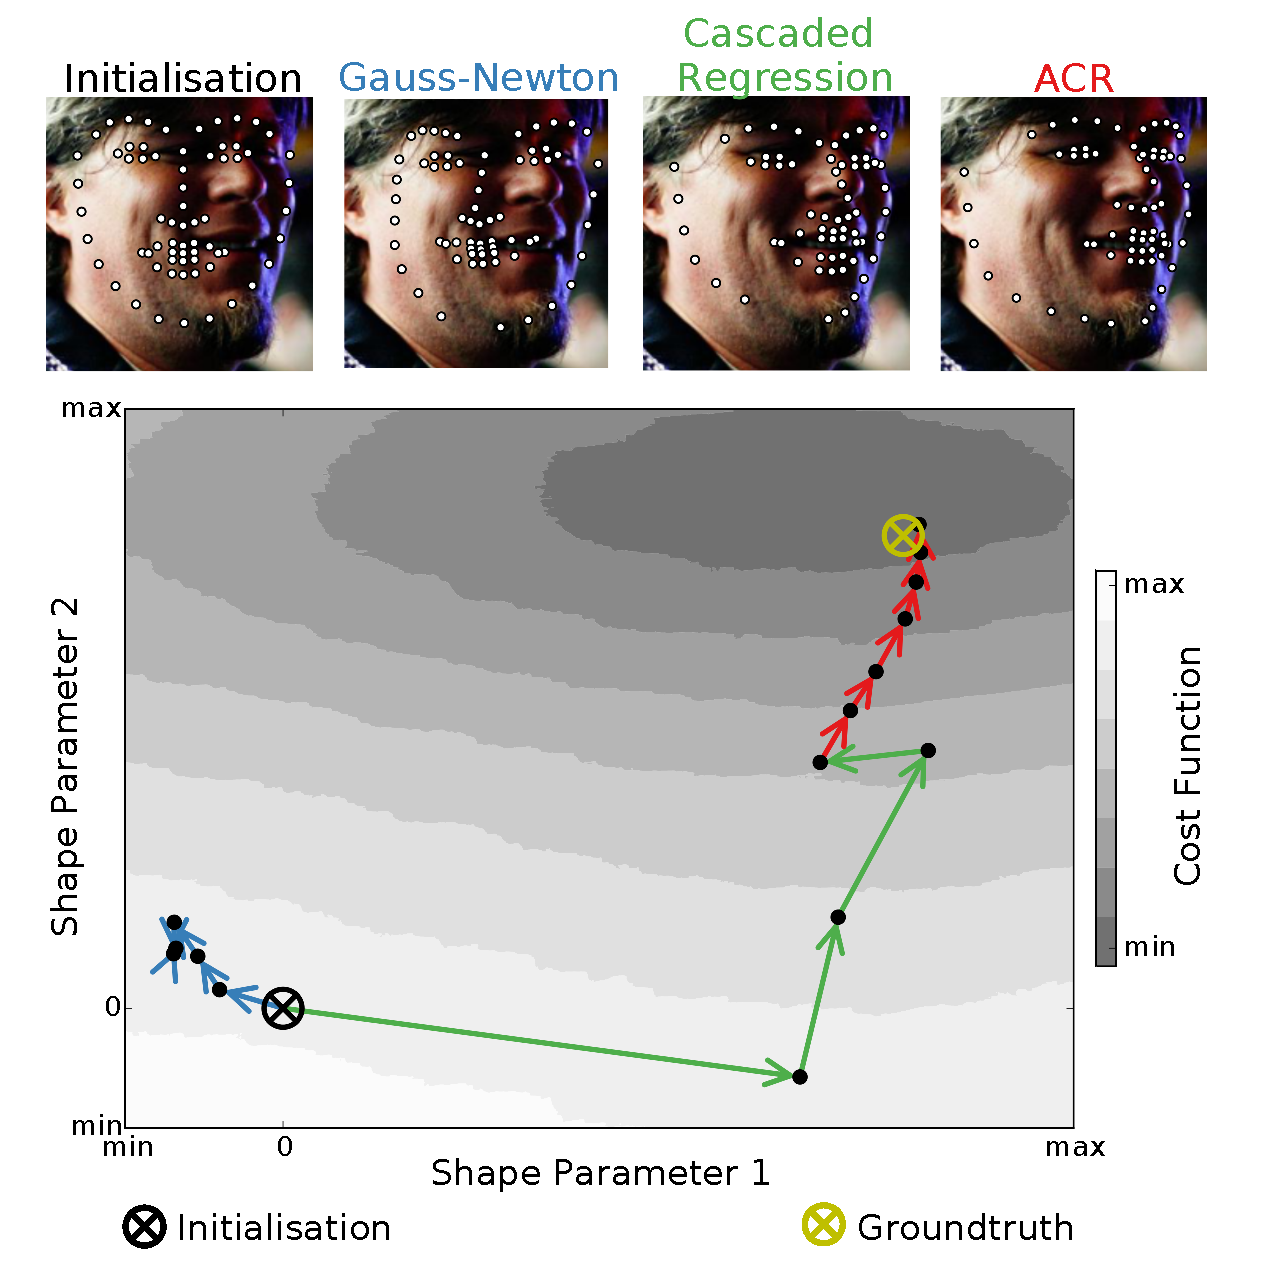
\includegraphics[width=0.7\linewidth]{figures/acr/motivation/final.eps}
  \caption{Example of descent directions obtained through optimization. The cost function, which is based on a parametric shape and appearance model, is plotted with respect to the two first shape parameters. Cascaded-regression (\emph{green}) moves towards the correct direction but does not reach the optimum. Gauss-Newton (\emph{blue}) diverges due to hard initialization. However, applying Gauss-Newton right after the final regression step (\emph{red}) converges to the ground-truth optimum. Motivated by this behavior, we propose a unified model that combines the regression-based discriminative and Gauss-Newton generative formulations.}
  \label{fig:motivation}
\end{figure}
%%%%%%%%%%%%%%%%%%%%%%%%%%%%%%%%%%%%%%%%%%%%%%%%%%

In this chapter, we present a unified model that combines the generative and
discriminative formulation. Our motivation comes from the example of
Figure~\ref{fig:motivation}. In this example, we plot the cost function
that we aim to optimize based on a parametric shape model and a projected-out
appearance subspace~\cite{matthews2004active}. Note that the cost function is
common for the discriminative and the generative models (more details will be
given in Secs.~\ref{subsec:regression},~\ref{subsec:generative},
Eq.~\ref{equ:equivalent_solutions}).
The cost function is plotted with respect to the first two shape parameters.
We also draw the descent directions provided by cascaded regression, followed
by a Gauss-Newton optimization. Note that even though the initialization is
far from the ground-truth optimum, the cascaded regression manages to quickly
converge towards the correct direction, but is not able to actually reach the
optimum. By initializing the Gauss-Newton algorithm from the final result of
the cascaded regression, we manage to reach the local optimum that corresponds
to the ground-truth, which translates to a lower point-to-point error. On the
other hand, the application of Gauss-Newton directly from the initial point
completely diverges due to the large distance from the optimum.

Motivated by the experiment of Figure~\ref{fig:motivation}, we believe that the
best result can be achieved by combining the discriminative cascaded regression
with the iterative Gauss-Newton optimization within a unified model. Our
proposed model employs a fully parametric cascade of regression-based descent
directions, which are further adapted by the gradient descent directions
provided by the Hessian of the Gauss-Newton method. This adaptation allows the
model to be robust to very challenging initializations and to converge to the
local minimum which can recover accurate landmark localization for the fine
details of an object. Inspired by our method's nature, we name it
Adaptive Cascaded Regression (ACR).

In summary, the contributions of this chapter are:
\begin{itemize}
    \item We propose a Deformable Model that takes advantage of the best of both
          worlds: cascaded discriminative and generative models. Our model
          combines these two approaches under a natural unified formulation. To
          the best of our knowledge, this is the first attempt of combining
          these two optimization worlds under a single cost function.
    \item We show that our method overcomes the disadvantages of both cascaded
          regression and Gauss-Newton optimization and exploits their strengths
          in terms of accuracy and convergence.
    \item We report state-of-the-art performance on the task of face alignment,
          using the most recent benchmark challenge
          300-W~\cite{sagonas2013semi,sagonas2013300,sagonas2016faces}.
\end{itemize}

\noindent The content of this chapter is based on the following publication:
\begin{itemize}
  \item \textbf{E. Antonakos}\textsuperscript{\ref{equal_authors}}, P. Snape\textsuperscript{\ref{equal_authors}}, G. Trigeorgis, and S. Zafeiriou.
  ``Adaptive Cascaded Regression'',
  \emph{Proceedings of IEEE International Conference on Image Processing (ICIP)},
  Phoenix, AZ, USA, \emph{Oral}, September 2016.
\end{itemize}

The rest of the chapter is structured as follows: Section~\ref{sec:acr:method}
first presents the discriminative approach (Sec.~\ref{subsec:regression}) and
then the generative one, in order to formulate the proposed model
(Sec.~\ref{subsec:acr}). Section~\ref{sec:acr:experiments} shows extended
experimental results and proves the state-of-the-art performance of the
proposed Deformable Model. Finally, Section~\ref{sec:acr:conclusion} concludes
the chapter.
